\begin{pastexam}[label={px:ncu-107-dsa-03}]{中央資工所 107 學年度 第 3 題}
（單選；每題 4 分，答錯倒扣一分）

The following statements S$_\mathrm{A}$ and S$_\mathrm{B}$ about minimum spanning tree (MST) may
not be correct. Assume that the weighted graph $G=(V,E)$ is undirected and connected. Do not
assume that edge weights are distinct unless this is specifically stated. Consider the following
two statements:

S$_\mathrm{A}$: If the lightest edge in $G$ is unique, then it must be part of every MST of $G$.\\
S$_\mathrm{B}$: If $G$ has a cycle with a unique lightest edge $e$, then $e$ must be part of
every MST of $G$.

(a)~Both S$_\mathrm{A}$ and S$_\mathrm{B}$ are false.\\
(b)~Both S$_\mathrm{A}$ and S$_\mathrm{B}$ are true.\\
(c)~S$_\mathrm{A}$ is true and S$_\mathrm{B}$ is false.\\
(d)~S$_\mathrm{A}$ is false and S$_\mathrm{B}$ is true.
\end{pastexam}

\begin{pastsoln}
答案是 (c)。

\textbf{S$_\mathrm{A}$ 對}。 設 $e = (u, v)$ 是 $G$ 裡唯一最輕的邊，也就是其他每條邊都比 $e$ 重。 假設
有一棵最小生成樹 $T$ 不含 $e$。 把 $e$ 加進 $T$，會和 $T$ 上 $u$ 到 $v$ 的路徑形成一個環；這個環上
除了 $e$ 還有別的邊，取其中一條 $e'$，$w(e') > w(e)$。 $T' = T + e - e'$ 仍然連通、有
$|V| - 1$ 條邊，是生成樹，而且 $w(T') = w(T) + w(e) - w(e') < w(T)$，和 $T$ 最小矛盾。 所以每一棵
最小生成樹都含 $e$。 這也是切割性質（資結書定理~24.1 和系理~24.2）的特例：取只含 $u$ 的切割，$e$
是跨過它唯一最輕的邊。

\textbf{S$_\mathrm{B}$ 錯}。 「環上最輕」不代表什麼；資結書定理~24.3 的環性質講的是環上\textbf{最重}
的邊。 反例：
\begin{center}
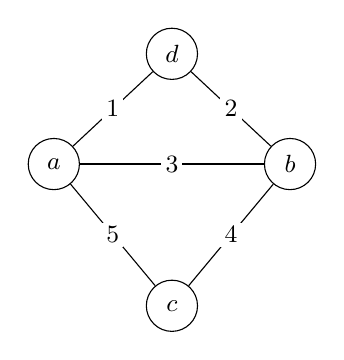
\begin{tikzpicture}[v/.style={circle,draw,minimum size=6.5mm,inner sep=0pt,font=\small},
    w/.style={fill=white,inner sep=1.5pt,font=\small}]
\node[v] (a) at (0,0) {$a$};
\node[v] (b) at (3,0) {$b$};
\node[v] (c) at (1.5,-1.8) {$c$};
\node[v] (d) at (1.5,1.4) {$d$};
\draw (a)--node[w]{3}(b);
\draw (b)--node[w]{4}(c);
\draw (a)--node[w]{5}(c);
\draw (a)--node[w]{1}(d);
\draw (d)--node[w]{2}(b);
\end{tikzpicture}
\end{center}
環 $a$--$b$--$c$--$a$ 的三條邊是 $3, 4, 5$，最輕的 $e = (a, b)$ 是唯一的。 但用 Kruskal（資結書
第~24.2~節）：先加 $ad$（$1$）、$db$（$2$）；$ab$（$3$）的兩端已經連通，跳過；再加 $bc$（$4$），
得到 $\{ad, db, bc\}$，總權重 $7$。 五條邊權重都不同，最小生成樹只有這一棵（資結書定理~24.4），
它不含 $e$。 直接比較也行：含 $ab$ 的生成樹最輕是 $ab + ad + bc = 3 + 1 + 4 = 8 > 7$。 原因是
$a$、$b$ 之間有一條更輕的路 $a$--$d$--$b$，$ab$ 在環 $a$--$d$--$b$--$a$ 上反而是最重的，由環性質
一定不在最小生成樹裡。

逐項檢查：(a) 說 S$_\mathrm{A}$ 錯、(b) 說 S$_\mathrm{B}$ 對、(d) 兩個都說反了，都錯；(c) 對。
\end{pastsoln}
